\documentclass[../../main.tex]{subfiles}

\graphicspath{{../../image/}{../../figure/}}

\begin{document}

\section{序列模型}\label{section:ch11-序列模型}

机器学习有许多重要的应用，其中的数据都由一系列的值组成，称为序列数据。例如，文本由一系列单词组成，而蛋白质则由一系列氨基酸组成。序列数据通常是按时间排序的，例如麦克风的音频信号或特定地点的日降雨量。有时，“时间”“过去”“未来”等术语也可以用于描述其他类型的序列数据，而不仅仅是时间序列。涉及序列数据的应用包括语音识别、不同语言间的自动翻译、DNA中的基因检测、合成音乐、编写计算机代码、与现代搜索引擎进行对话等。

我们用$x_1,\cdots,x_N$表示序列数据，其中的每个元素$x_n$都包含一个值向量。请注意，我们可能会有好几个这样的序列数据（后文简称序列），它们分别独立地取自同一个分布。在这种情况下，所有序列的联合分布可以分解为每个序列分布的乘积。由此，我们可以仅关注其中一个序列的建模。

根据\eqref{align:ch11-K变量分解}，我们已经看到，通过反复应用概率的乘积法则，$N$个变量的一般分布可以写成条件分布的乘积，而这种分解的形式取决于变量的特定排序。对于向量值变量，如果我们选择与序列中变量顺序相对应的排序，则可以写出
\begin{align}
  p(x_1,\cdots,x_N) = \prod_{n=1}^{N}p(x_n\mid x_1,\cdots,x_{n-1}),
  \label{align:ch11-自回归一般分解}
\end{align}
这对应于一个有向图，其中每个节点都从序列中的每个前一节点接收一个连接，如\cref{figure:ch11-自回归模型}中的4个节点所示。

\begin{definition}[自回归模型]\label{definition:ch11-自回归}
若序列的联合分布按\eqref{align:ch11-自回归一般分解}分解，即每个条件分布以序列中它之前的全部变量为条件，则称该模型为\textbf{自回归}（autoregressive）模型。由\cref{proposition:ch11-有向图分解}，\eqref{align:ch11-自回归一般分解}的每个因子都是归一化的条件分布，因此该分解对任意序列分布都成立。
\end{definition}

% SUPPLEMENT: parent=definition:ch11-自回归; kind=motivation; location=紧随其后的 remark（重构新增）
\begin{remark}（重构新增）
\cref{definition:ch11-自回归}的分解与\eqref{align:ch11-K变量分解}是同一个式子，只是把“变量”换成了“序列的元素”，并把排序固定为时间顺序。这一排序的选择是有代价的：它假定了“第$n$个元素只依赖过去”这一非对称的建模方向，因此自回归模型不能直接表示“未来的观测影响过去的观测”这类依赖。另一方面，一般性也是它的弱点：\eqref{align:ch11-自回归一般分解}对任何分布都成立，因此它本身不表达任何假设，参数数量随$N$指数增长，必须通过后面的 Markov 假设或参数共享（\cref{definition:ch11-共享参数}）加以限制。
\end{remark}

\begin{figure}[htbp]
  \centering
  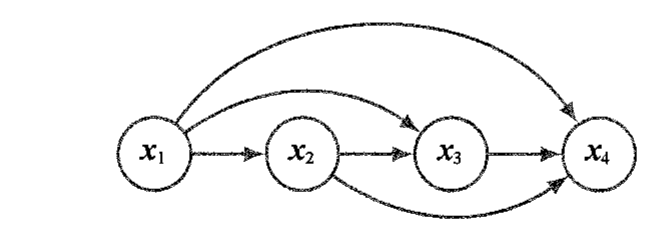
\includegraphics[width=0.62\textwidth]{ch11-fig11-27-autoregressive.png}
  \caption{具有4个节点且形式为\eqref{align:ch11-自回归一般分解}的一般自回归模型的示意图}
  \label{figure:ch11-自回归模型}
\end{figure}

这种表示法具有完全的通用性，因此从建模的角度来看没有任何价值，因为它没有表达任何假设。我们可以通过从图中移除连接，或者等效地从\eqref{align:ch11-自回归一般分解}右侧因子的条件集中去除变量，来引入条件独立性，从而限制模型的空间。

最有力的假设是去除所有条件变量，从而得出联合分布，其形式为
\begin{align}
  p(x_1,\cdots,x_N) = \prod_{n=1}^{N}p(x_n).
  \label{align:ch11-独立序列}
\end{align}

\eqref{align:ch11-独立序列}将观测变量视为独立变量，因此完全忽略了排序信息。这对应于一个无连接的概率图模型，如\cref{figure:ch11-独立变量图模型}所示。

\begin{figure}[htbp]
  \centering
  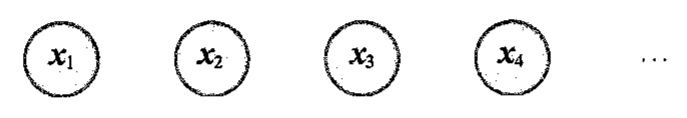
\includegraphics[width=0.60\textwidth]{ch11-fig11-28-independent.png}
  \caption{对一系列观测变量进行建模的最简单方法是将其视为独立变量，这对应于一个无连接的图模型}
  \label{figure:ch11-独立变量图模型}
\end{figure}

既能捕获到顺序特性，又能引入建模假设的有趣模型介于以上两个极端之间。一个强有力的假设是，每个条件分布都只依赖于序列中的前一个变量，从而得出如下联合分布：
\begin{align}
  p(x_1,\cdots,x_N) = p(x_1)\prod_{n=2}^{N}p(x_n\mid x_{n-1}).
  \label{align:ch11-一阶Markov}
\end{align}

请注意，序列中第一个变量的处理方式略有不同，因为它没有条件变量。\cref{figure:ch11-一阶Markov链}所示图模型的函数形式[\eqref{align:ch11-一阶Markov}]称为Markov模型或Markov链，其可用简单节点链组成的图来表示。

\begin{definition}[$M$阶Markov模型]\label{definition:ch11-Markov模型}
若序列的联合分布可写成
\begin{align}
  p(x_1,\cdots,x_N) = p(x_1,\cdots,x_M)\prod_{n=M+1}^{N}p(x_n\mid x_{n-M},\cdots,x_{n-1}),
  \label{align:ch11-M阶Markov}
\end{align}
则称其为\textbf{$M$阶Markov模型}（$M$-th order Markov model），其中每个条件分布只依赖前面$M$个变量。$M=1$时\eqref{align:ch11-M阶Markov}退化为\eqref{align:ch11-一阶Markov}，称为\textbf{一阶Markov模型}或\textbf{Markov链}；$M=2$时称为二阶Markov模型。
\end{definition}

% SUPPLEMENT: parent=definition:ch11-Markov模型; kind=motivation; location=紧随其后的 remark（重构新增）
\begin{remark}（重构新增）
\cref{definition:ch11-Markov模型}的关键是“阶数”$M$：它规定了条件分布的记忆长度，从而把\eqref{align:ch11-自回归一般分解}中第$n$个因子的条件集从$n-1$个变量削减到$M$个。前$M$个变量需要单独处理，因为它们的条件变量不足$M$个，这不是技术细节而是定义的一部分：若强行对$n\leqslant M$使用同一个条件分布，就需要引入“虚拟的”过去值。$M$的选择直接决定模型的表达能力与参数规模，二者由\cref{proposition:ch11-序列参数计数}定量刻画。另请注意，$M$阶Markov性是对联合分布的一个约束，而不是对单个条件分布的约束；它等价于说“给定最近$M$个观测，更早的观测不再提供信息”。
\end{remark}

\begin{figure}[htbp]
  \centering
  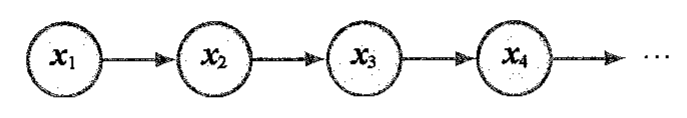
\includegraphics[width=0.60\textwidth]{ch11-fig11-29-first-order-chain.png}
  \caption{观测值的一阶Markov链，其中特定观测值$x_n$的分布以前一个观测值$x_{n-1}$为条件}
  \label{figure:ch11-一阶Markov链}
\end{figure}

通过使用d分离（参见\cref{subsection:ch11-d分离}），我们可以看到，在时间$n$之前的所有观测值中，观测值$x_{n-1}$的条件分布为
\begin{align}
  p(x_n\mid x_1,\cdots,x_{n-1}) = p(x_n\mid x_{n-1}).
  \label{align:ch11-一阶Markov性质}
\end{align}

\begin{proposition}[一阶Markov性质]\label{proposition:ch11-一阶Markov性质}
设$p(x_1,\cdots,x_N)$由\eqref{align:ch11-一阶Markov}给出，则对$n=2,\cdots,N$，\eqref{align:ch11-一阶Markov性质}成立，即
\begin{align}
  x_n \perp \{x_1,\cdots,x_{n-2}\} \mid x_{n-1},
\end{align}
其中约定$n=2$时$\{x_1,\cdots,x_{n-2}\}$为空集（此时条件独立性平凡成立）。
\end{proposition}

\begin{proof}
（重构新增）由乘积法则与\eqref{align:ch11-一阶Markov}，
\begin{align}
  p(x_n\mid x_1,\cdots,x_{n-1}) = \frac{p(x_1,\cdots,x_n)}{p(x_1,\cdots,x_{n-1})}
  = \frac{p(x_1)\prod_{m=2}^{n}p(x_m\mid x_{m-1})}{p(x_1)\prod_{m=2}^{n-1}p(x_m\mid x_{m-1})} = p(x_n\mid x_{n-1}),
\end{align}
分子分母中$m\leqslant n-1$的因子逐一相消，只剩最后一个因子。这同时说明$x_n$与$x_1,\cdots,x_{n-2}$在给定$x_{n-1}$后条件独立（见\cref{exercise:ch11-16}）。
\end{proof}

% SUPPLEMENT: parent=proposition:ch11-一阶Markov性质; kind=motivation; location=紧随其后的 remark（重构新增）
\begin{remark}（重构新增）
\cref{proposition:ch11-一阶Markov性质}给出了两种等价的验证方式：代数上靠因子相消，图形上靠d分离（路径$x_n\to x_{n-1}\to\cdots\to x_1$在$x_{n-1}$处头尾相接且$x_{n-1}$已观测，故被阻塞）。相消过程中分子分母必须“逐因子对齐”，这依赖\eqref{align:ch11-一阶Markov}的乘积顺序与时间顺序一致；若把序列倒序写出，因子形式改变，但条件独立性的结论不变。该性质是“用前一个观测预测下一个观测”的全部理论依据，因此在实际预测中，只要模型是一阶Markov的，就可以丢弃$x_{n-2}$及更早的全部历史。
\end{remark}

从\eqref{align:ch11-一阶Markov性质}开始，利用概率的乘积法则，直接求值即可对此轻松验证（见\cref{exercise:ch11-16}）。因此，如果我们使用这样一个模型来预测序列中的下一个观测值，则预测值的分布将只取决于前一个观测值，而与之前的所有观测值无关。

更具体地说，形式为\eqref{align:ch11-一阶Markov}的图模型称为一阶Markov模型，因为每个条件分布中只出现了一个条件变量。我们可以对这个模型进行扩展，方法是让每个条件分布都依赖于前面的两个变量，从而得到一个二阶Markov模型，其形式为
\begin{align}
  p(x_1,\cdots,x_N) = p(x_1)\,p(x_2\mid x_1)\prod_{n=3}^{N}p(x_n\mid x_{n-1},x_{n-2}).
  \label{align:ch11-二阶Markov}
\end{align}

请注意，前两个变量的处理方法不同，因为它们的条件变量少于两个。\cref{figure:ch11-二阶Markov链}以有向图的形式对该模型进行了展示。

\begin{figure}[htbp]
  \centering
  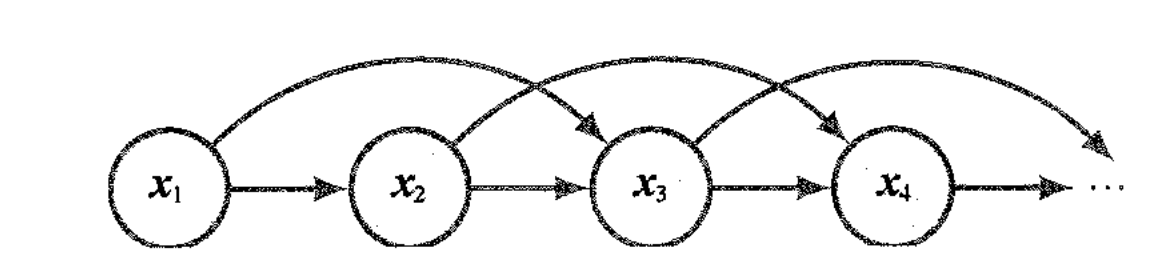
\includegraphics[width=0.66\textwidth]{ch11-fig11-30-second-order-chain.png}
  \caption{一个二阶Markov链，其中特定观测值$x_n$的条件分布取决于前两个观测值$x_{n-1}$和$x_{n-2}$}
  \label{figure:ch11-二阶Markov链}
\end{figure}

通过使用d分离（或使用概率规则进行直接计算），我们可以看到，在二阶Markov模型中，给定所有先前观测值$x_1,\cdots,x_{n-1}$的$x_n$的条件分布与观测值$x_1,\cdots,x_{n-3}$无关（见\cref{exercise:ch11-17}）。同样，我们可以考虑扩展到$M$阶Markov链，其中某个变量的条件分布取决于前$M$个变量。

假设观测值是具有$K$种状态的离散变量，此时一阶Markov链中的条件分布$p(x_n\mid x_{n-1})$将由一组参数（共$K-1$个）指定；在$x_{n-1}$的$K$个状态中，每个状态都有$K-1$个参数，共有$K(K-1)$个参数。假设我们将模型扩展为$M$阶Markov模型，这样联合分布便可用条件式$p(x_n\mid x_{n-M},\cdots,x_{n-1})$来构造。如果变量是离散的且条件分布用一般条件概率来表示，模型将有$K^{M-1}(K-1)$个参数。因此，参数数量会随着$M$的增加而呈指数增长，一般来说，$M$的值越大，这种方法就越不实用。

\begin{proposition}[$M$阶Markov模型的参数计数]\label{proposition:ch11-序列参数计数}
设观测值为$K$状态的离散变量，条件分布用完整条件概率表给出。则$M$阶Markov模型\eqref{align:ch11-M阶Markov}中，每个条件分布$p(x_n\mid x_{n-M},\cdots,x_{n-1})$需要$K^{M}(K-1)$个自由参数，整个模型（忽略前$M$个变量的初始分布）需要$K^{M}(K-1)$个转移参数。
\end{proposition}

\begin{proof}
（重构新增）条件分布$p(x_n\mid x_{n-M},\cdots,x_{n-1})$对条件变量的每个取值组合给出一个长度为$K$的概率向量。条件变量共有$M$个、每个$K$种取值，故共有$K^{M}$个组合；每个概率向量受归一化约束，只有$K-1$个自由参数。相乘得$K^{M}(K-1)$。$M=1$时它等于$K(K-1)$，与正文中一阶链的参数数目一致；$M=0$时它退化为$K-1$，即无记忆的独立模型。前$M$个变量的初始分布$p(x_1,\cdots,x_M)$另需$K^{M}-1$个参数，正文所说的“构造联合分布所需的参数”通常只统计随$n$重复使用的转移参数。
\end{proof}

% SUPPLEMENT: parent=proposition:ch11-序列参数计数; kind=motivation; location=紧随其后的 remark（重构新增）
\begin{remark}（重构新增）原文问题说明
原文把$M$阶模型的参数数目印作$K^{M-1}(K-1)$，这与同一段前面给出的“一阶链共有$K(K-1)$个参数”相矛盾：代入$M=1$会得到$K-1$，而不是$K(K-1)$。按\cref{proposition:ch11-序列参数计数}的推导，正确数目是$K^{M}(K-1)$，它在$M=1$时给出$K(K-1)$，在$M=0$时给出$K-1$，两个端点都吻合。因此这里按修正后的$K^{M}(K-1)$理解。无论采用哪个式子，结论“参数随$M$指数增长”都不变，这也是高阶Markov模型在实践中很少直接使用的根本原因；替代方案是\cref{definition:ch11-状态空间模型}的潜变量模型，它用$O(K^2)$个转移参数换取任意长的记忆。
\end{remark}

\subsection*{潜变量}

假设我们希望为序列建立一个模型，这个模型不受Markov假设的任何顺序的限制，但可以使用有限数量的自由参数来指定。我们可以通过引入额外的潜变量（又称隐变量）来实现这一目标，从而允许从简单组件中构建出类别丰富的模型。对于每个观测值$x_n$，我们引入一个相应的潜变量$z_n$（可能与观测变量的类型或维度不同）。现在，我们假设潜变量构成了Markov链，从而产生了状态空间模型的图结构，如\cref{figure:ch11-状态空间模型}所示。它满足关键的条件独立性要求，即给定$z_n$时，$z_{n-1}$和$z_{n+1}$是独立的，因此
\begin{align}
  z_{n+1} \perp z_{n-1} \mid z_n.
  \label{align:ch11-状态空间条件独立}
\end{align}

\begin{definition}[状态空间模型]\label{definition:ch11-状态空间模型}
设$z_1,\cdots,z_N$是潜变量，$x_1,\cdots,x_N$是观测变量，且联合分布按有向\cref{figure:ch11-状态空间模型}分解为
\begin{align}
  p(x_1,\cdots,x_N,z_1,\cdots,z_N) = p(z_1)\left[\prod_{n=2}^{N}p(z_n\mid z_{n-1})\right]\left[\prod_{n=1}^{N}p(x_n\mid z_n)\right],
  \label{align:ch11-状态空间联合}
\end{align}
则称该模型为\textbf{状态空间模型}（state space model）。其中$p(z_1)$是初始分布，$p(z_n\mid z_{n-1})$是转移分布，$p(x_n\mid z_n)$是发射分布。
\end{definition}

% SUPPLEMENT: parent=definition:ch11-状态空间模型; kind=motivation; location=紧随其后的 remark（重构新增）
\begin{remark}（重构新增）
\cref{definition:ch11-状态空间模型}用“潜变量链+逐点发射”替换了\eqref{align:ch11-M阶Markov}的“显式记忆$M$步”。这样做的收益是参数数量与$N$无关、且记忆长度不受限制；代价是观测变量之间不再有直接的边，所有依赖都必须通过潜状态传递，因此似然需要对潜变量求积分（求和），一般无法解析计算。\eqref{align:ch11-状态空间联合}的三部分——初始、转移、发射——正是隐Markov模型与线性动态系统的共同骨架，二者的区别仅在于$z_n$是离散还是连续、发射分布是离散表还是线性Gauss（\cref{definition:ch11-线性Gauss模型}）。这种“同一图、不同分布族”的现象再次说明图结构与分布族是两个独立的建模维度。
\end{remark}

\begin{figure}[htbp]
  \centering
  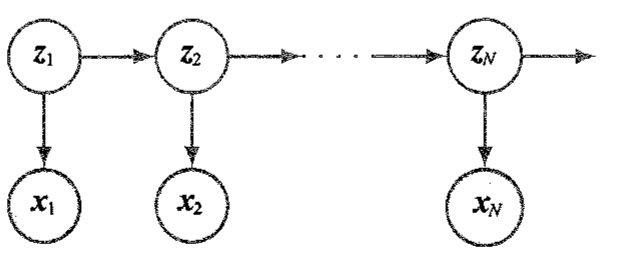
\includegraphics[width=0.58\textwidth]{ch11-fig11-31-state-space.png}
  \caption{状态空间模型用潜变量$z_1,\cdots,z_N$表示一系列观测变量$x_1,\cdots,x_N$的联合概率分布，它的形式如\eqref{align:ch11-状态空间联合}所示}
  \label{figure:ch11-状态空间模型}
\end{figure}

通过使用d分离，我们可以发现，在状态空间模型中，总有一条路径能通过潜变量连接任意两个观测变量$x_i$和$x_m$，而且这条路径永远不会阻塞。因此，在给定所有先前观测值的情况下，观测值$x_{n+1}$的预测分布$p(x_{n+1}\mid x_1,\cdots,x_n)$并不会表现出任何条件独立性，因此我们对$x_{n+1}$的预测取决于所有先前的观测值。观测变量在任何有限阶（order）都不符合Markov特性。

\cref{figure:ch11-状态空间模型}描述了两个重要的序列模型。如果潜变量是离散的，我们就会得到一个隐Markov模型（Elliott, Aggoun, and Moore, 1995）。请注意，隐Markov模型中的观测变量既可以是离散的，也可以是连续的，而且可以使用多种不同的条件分布来进行建模。如果潜变量和观测变量都是Gauss变量（其条件分布与父变量之间存在线性-Gauss依赖关系），我们就可以得到一个线性动态系统，也称Kalman滤波器（Zarchan and Musoff, 2005）。Bishop (2006) 详细讨论了隐Markov模型和Kalman滤波器，以及训练它们的算法。用深度神经网络取代用于定义$p(x_n\mid z_n)$的简单离散概率表或线性Gauss分布，便可以使这类模型变得更加灵活。

\begin{definition}[隐Markov模型]\label{definition:ch11-隐Markov模型}
在\cref{definition:ch11-状态空间模型}中，若潜变量$z_n$取$K$个离散状态且转移与发射都是离散分布，则称该模型为\textbf{隐Markov模型}（hidden Markov model, HMM）。若$z_n$与$x_n$都是Gauss变量且条件分布是线性Gauss的，则称该模型为\textbf{线性动态系统}（linear dynamical system），也称\textbf{Kalman滤波器}。
\end{definition}

% SUPPLEMENT: parent=definition:ch11-隐Markov模型; kind=motivation; location=紧随其后的 remark（重构新增）
\begin{remark}（重构新增）
\cref{definition:ch11-隐Markov模型}中“隐”字指状态$z_n$不可观测，只有$x_n$可见；这与\cref{definition:ch11-Markov模型}的（显式）Markov链形成对比：后者的状态就是观测本身。HMM的表达能力来自“离散状态+任意发射分布”的组合：状态转移只有$K^2$个参数，而发射分布$p(x_n\mid z_n)$可以是离散表、Gauss密度，甚至可以是由深度神经网络参数化的分布（此时模型常称为神经HMM）。需要注意，HMM的似然$p(x_1,\cdots,x_N)$需要对$K^N$条状态路径求和，直接计算不可行，必须使用下面的前向–后向递推。
\end{remark}

\begin{remark}（重构新增）
原书在此只给出了状态空间模型与HMM的图结构和定义，并把前向–后向算法与参数学习留给了 Bishop (2006)。为使本章的序列模型部分自足，下面补写HMM的似然计算与前向–后向递推，以下内容均为重构新增，不冒充原书内容。
\end{remark}

\begin{proposition}[HMM的前向--后向递推（重构新增）]\label{proposition:ch11-前向后向}
设$p(z_1,\cdots,z_N,x_1,\cdots,x_N)$由\eqref{align:ch11-状态空间联合}给出，$z_n\in\{1,\cdots,K\}$。定义\textbf{前向变量}与\textbf{后向变量}
\begin{align}
  \alpha_n(z_n) &\triangleq p(x_1,\cdots,x_n,z_n),\\
  \beta_n(z_n) &\triangleq p(x_{n+1},\cdots,x_N\mid z_n).
\end{align}
则它们满足递推
\begin{align}
  \alpha_1(z_1) &= p(z_1)\,p(x_1\mid z_1),\qquad
  \alpha_n(z_n) = p(x_n\mid z_n)\sum_{z_{n-1}}\alpha_{n-1}(z_{n-1})\,p(z_n\mid z_{n-1}),
  \label{align:ch11-前向递推}\\
  \beta_N(z_N) &= 1,\qquad
  \beta_n(z_n) = \sum_{z_{n+1}}\beta_{n+1}(z_{n+1})\,p(x_{n+1}\mid z_{n+1})\,p(z_{n+1}\mid z_n),
  \label{align:ch11-后向递推}
\end{align}
并且对任意$n=1,\cdots,N$，似然可写成
\begin{align}
  p(x_1,\cdots,x_N) = \sum_{z_N}\alpha_N(z_N) = \sum_{z_n}\alpha_n(z_n)\,\beta_n(z_n),
  \label{align:ch11-似然前向后向}
\end{align}
潜状态的后验边缘为
\begin{align}
  \gamma_n(z_n) \triangleq p(z_n\mid x_1,\cdots,x_N) = \frac{\alpha_n(z_n)\,\beta_n(z_n)}{p(x_1,\cdots,x_N)}.
  \label{align:ch11-后验边缘}
\end{align}
\end{proposition}

\begin{proof}
（重构新增）前向递推：由乘积法则与\eqref{align:ch11-状态空间联合}，$p(x_1,\cdots,x_n,z_n)$可以写成“前$n-1$步的全部变量”与“第$n$步”的乘积，并对$z_{n-1}$求和：
\begin{align}
  \alpha_n(z_n) &= \sum_{z_{n-1}}p(x_1,\cdots,x_n,z_{n-1},z_n)
  = \sum_{z_{n-1}}p(x_1,\cdots,x_{n-1},z_{n-1})\,p(z_n\mid z_{n-1})\,p(x_n\mid z_n)\\
  &= p(x_n\mid z_n)\sum_{z_{n-1}}\alpha_{n-1}(z_{n-1})\,p(z_n\mid z_{n-1}),
\end{align}
其中第二个等号用了条件独立性：给定$z_{n-1},z_n$后，$(x_1,\cdots,x_{n-1})$与$(x_n,z_n)$独立（\cref{figure:ch11-状态空间模型}中路径在$z_n$处被观测节点$z_n$阻塞）。基例$\alpha_1(z_1)=p(z_1)p(x_1\mid z_1)$由同一分解直接得到。

后向递推：对$z_{n+1}$用全概率公式并再次利用条件独立性，
\begin{align}
  \beta_n(z_n) &= \sum_{z_{n+1}}p(x_{n+1},\cdots,x_N,z_{n+1}\mid z_n)
  = \sum_{z_{n+1}}p(z_{n+1}\mid z_n)\,p(x_{n+1}\mid z_{n+1})\,p(x_{n+2},\cdots,x_N\mid z_{n+1})\\
  &= \sum_{z_{n+1}}p(z_{n+1}\mid z_n)\,p(x_{n+1}\mid z_{n+1})\,\beta_{n+1}(z_{n+1}),
\end{align}
基例$\beta_N(z_N)=p(\varnothing\mid z_N)=1$。

似然：$\alpha_N(z_N)=p(x_1,\cdots,x_N,z_N)$，对$z_N$求和即得第一个等号；另一方面，对任意$n$，
\begin{align}
  \alpha_n(z_n)\beta_n(z_n)=p(x_1,\cdots,x_n,z_n)\,p(x_{n+1},\cdots,x_N\mid z_n)=p(x_1,\cdots,x_N,z_n),
\end{align}
其中用了给定$z_n$时“过去”与“未来”条件独立。对$z_n$求和即得\eqref{align:ch11-似然前向后向}的第三个等号。

后验边缘：由Bayes定理，$p(z_n\mid x_1,\cdots,x_N)=p(x_1,\cdots,x_N,z_n)/p(x_1,\cdots,x_N)$，分子即上式，代回即得\eqref{align:ch11-后验边缘}。
\end{proof}

% SUPPLEMENT: parent=proposition:ch11-前向后向; kind=motivation; location=紧随其后的 remark（重构新增）
\begin{remark}（重构新增）
\cref{proposition:ch11-前向后向}的核心是“动态规划”：直接计算似然要对$K^N$条状态路径求和，而\eqref{align:ch11-前向递推}把求和按时间分解，每一步只保留$K$个数，总代价为$O(NK^2)$（每个$n$要做$K^2$次乘加），从指数级降到线性级。这一“把路径求和改写为逐时刻状态求和”的技巧与\cref{subsection:ch11-作为过滤器的图}中消息传递的思想完全一致：前向变量就是沿链从过去传向未来的消息，后向变量是反向的消息。\eqref{align:ch11-似然前向后向}中“对任意$n$求和都得到同一个数”是算法正确性的自检条件，也是数值稳定化（缩放）的出发点：$\alpha_n$与$\beta_n$分别随$n$指数衰减与增长，实现时必须每步归一化。条件“$z_n$离散”保证了求和可算；若$z_n$连续（如Kalman滤波器），求和换成积分，线性Gauss情形下积分仍有闭式解，这正是\cref{proposition:ch11-线性Gauss矩}在Gauss情形下的对应物。
\end{remark}

\end{document}
